\documentclass[12pt]{book}
\usepackage[a6paper]{geometry}

% wegen deutschen Umlauten
\usepackage[utf8]{inputenc}
\usepackage[cmintegrals,cmbraces]{newtxmath}
\usepackage{ebgaramond-maths}
\usepackage[T1]{fontenc}

% deutsche Silbentrennung
\usepackage[ngerman]{babel}

% keine Einrückung am Beginn eines Absatzes:
\usepackage{parskip}

%%%%%%%%%%%%%%%%%%%%%%%%%%%%%%%%%%%%%%%%%%%%%%%%%%%%%%%%%%%%%%
% header / footer
\usepackage{fancyhdr}

% font size
\newcommand{\changefont}{%
    \fontsize{9}{11}\selectfont
}
\fancyhf{}
\fancyhead[LE,RO]{\changefont\slshape \rightmark} %section
\fancyhead[RE,LO]{\changefont\slshape \leftmark} %chapter
\fancyfoot[C]{\changefont\thepage} %footer
\pagestyle{fancy}

% header end
%%%%%%%%%%%%%%%%%%%%%%%%%%%%%%%%%%%%%%%%%%%%%%%%%%%%%%%%%%%%%%

\usepackage{graphicx}
\graphicspath{ {./bilder/a6/} }

% empty pages:
%\usepackage{afterpage}

% Wieviel cm ist \textwidth?
%\usepackage{layouts}
%textwidth in cm: \printinunitsof{cm}\prntlen{\textwidth}

%
\usepackage{blindtext}

\begin{document}

\frontmatter

\begin{titlepage}
	\centering
	%{\scshape\LARGE Columbidae University \par}
	%\vspace{1cm}
	%{\scshape\Large Final year project\par}
	\vspace{3cm}
	{\huge\bfseries Klassiker der Lyrik\par}
	\vspace{1.5cm}
	{\Large\itshape Dies und Das\par}
	\vfill
	2016 \par
	\textsc{89. Auflage}

	\vfill

% Bottom of the page
	%{\large \today\par}
\end{titlepage}

%textwidth in cm: \printinunitsof{cm}\prntlen{\textwidth}

%textheight in cm: \printinunitsof{cm}\prntlen{\textheight}

% for empty pages:
\mbox{}
\thispagestyle{empty}
\newpage

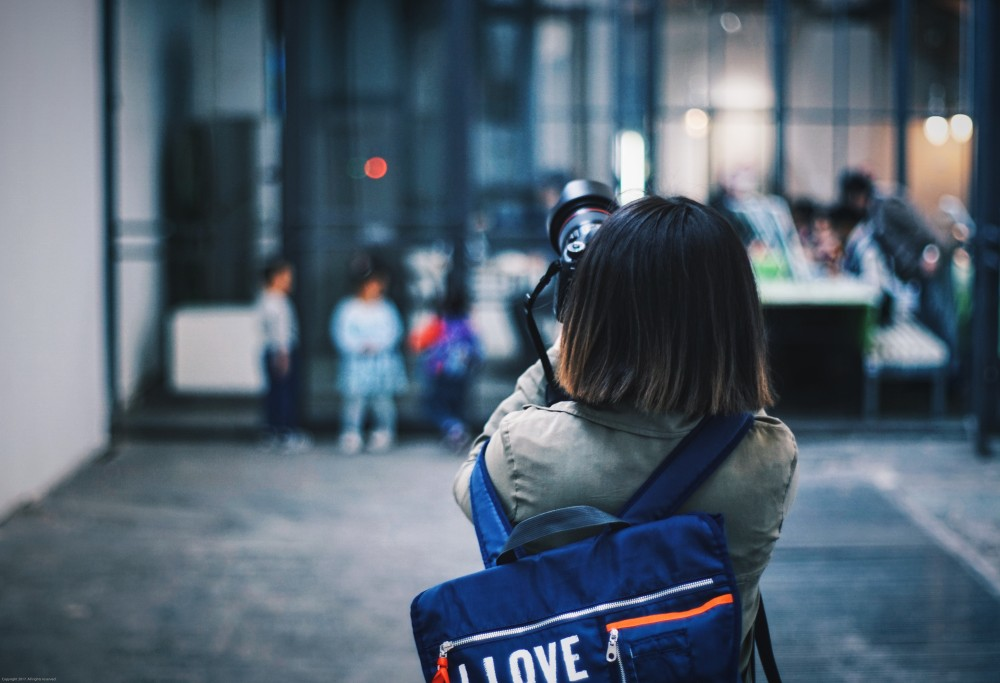
\includegraphics[width=1\textwidth]{images/photo1000.jpg}

\newpage

\tableofcontents

\mainmatter

\chapter{Anfang, Anfang}
\label{chap:Anfang, Anfang}

\blindtext[3]

\blindenumerate

\emph{Juli 2016}

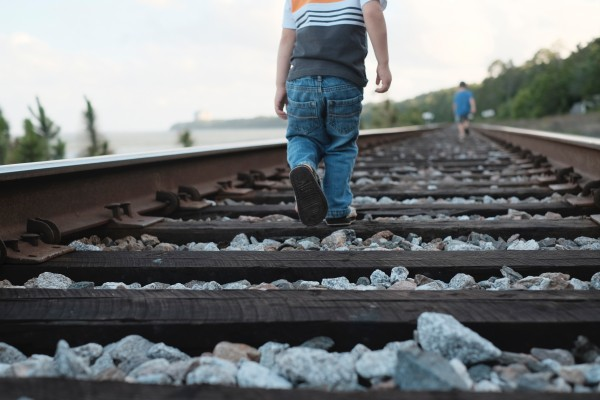
\includegraphics[width=1\textwidth]{images/gleis600x450.jpg}

\chapter{Immer weiter}
\label{chap:Immer weiter}

\Blindtext

\emph{Mai 2016}

\clearpage

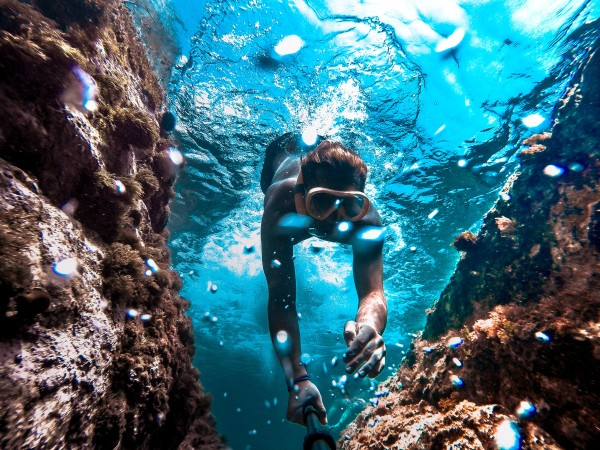
\includegraphics[width=1\textwidth]{images/dive600x450.jpg}

\chapter{Und weiter}
\label{chap:Und weiter}

\Blindtext

\emph{Januar 2016}

\clearpage

\chapter{Anhang}

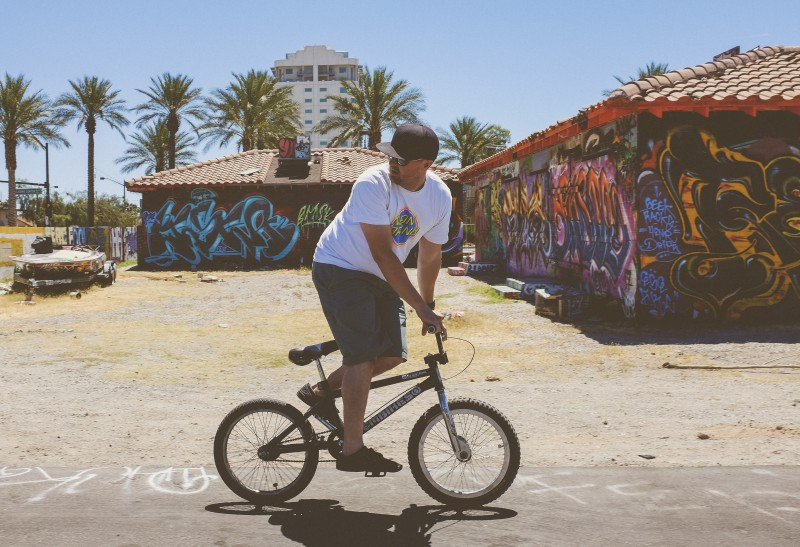
\includegraphics[width=1\textwidth]{images/bike800.jpg}

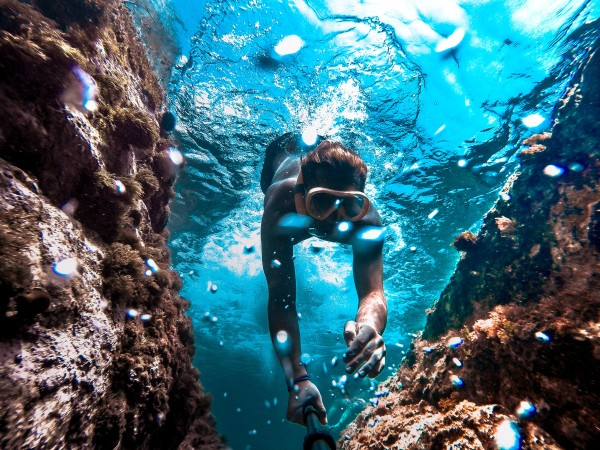
\includegraphics[width=1\textwidth]{images/dive600x450.jpg}

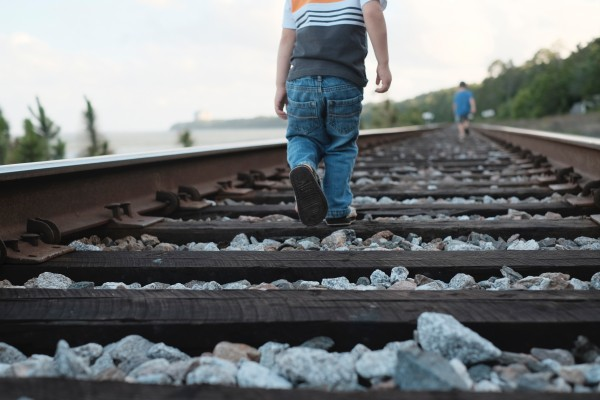
\includegraphics[width=1\textwidth]{images/gleis600x450.jpg}

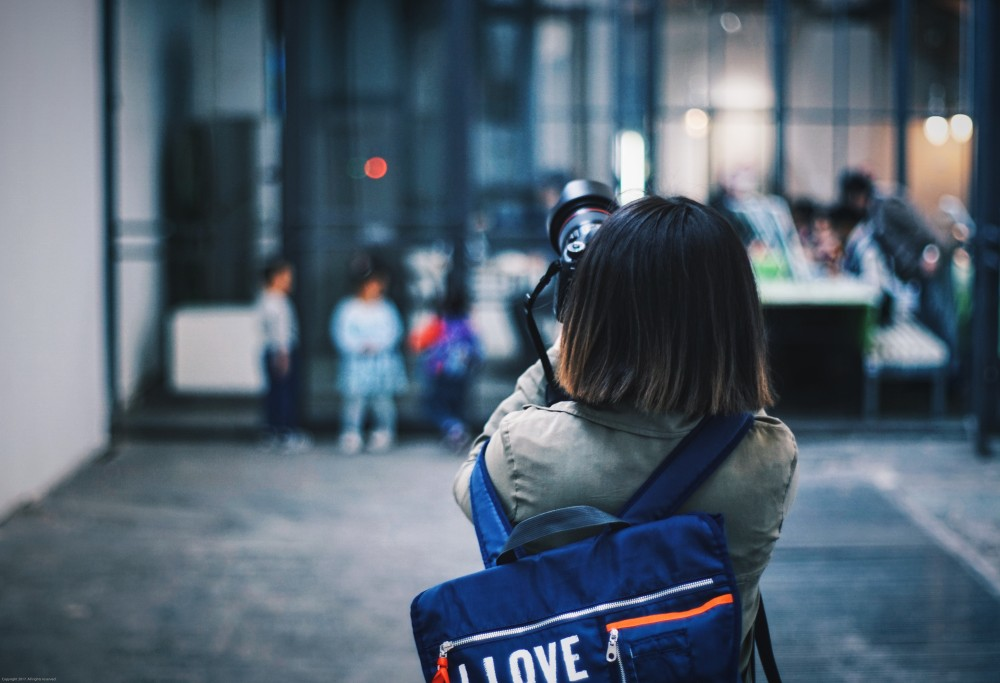
\includegraphics[width=1\textwidth]{images/photo1000.jpg}

\end{document}
